\documentclass[a4paper,12pt]{article}

\usepackage{fullpage} % Package to use full page
\usepackage{parskip} % Package to tweak paragraph skipping
% \usepackage{tikz} % Package for drawing
\usepackage{amsmath}
% \usepackage{amsfonts}
\usepackage{hyperref}
\usepackage{listings}
\usepackage{mathptmx}
\usepackage{tabularx}

\usepackage{setspace}
\doublespacing

\usepackage{graphicx}
\usepackage{subcaption}
\graphicspath{ {./pics/} }

\usepackage{float}
\floatstyle{boxed} 

\usepackage{natbib}

\title{Machine Learning Applied on Portfolio Optimization}
\author{Eric Wang}
\date{\today}

\renewcommand{\figurename}{Ffigwr}

\begin{document}

\maketitle

\section{Introduction}

This project is built with python and all of my codes can be accessed through my \href{https://github.com/ywang408/ml_portfolio_optimization}{github}. In this project, instead of using global Mean-Variance Optimization(MVO) strategy with a fixed window for re-allocating assets, I use a more flexible strategy to estimate expected return, covariance matrix and determine when to adjust the portfolio weights.

I try several unsupervised learning models to analyze the market regimes, and I find that K-means clustering with technical indicators outperforms the other models. To minimize the risk of my portfolio, I use all S\&P 500 component stocks as my stock pool. However, a very large dataset is required to estimate the expected return and covariance matrix of all 500 stocks, thus I use Support Vector Machine(SVM) to create a subset of stocks for investing before re-allocating my portfolio. I also use a shrinkage estimator for covariance matrix to make sure that it's positive definite such that optimization problem can be solved. At the end, I choose an proper optimization strategy to build my portfolio, results of backtesting shows that this strategy is practicable.

% This report is organized as following, in chapter 2, I discuss the process of handling data, how to use Gaussian Mixture Method and K-means method to analyze the market regime, and show the performance of using Support Vector Machine(SVM) to determine whether to invest a stock. In chapter 3, I will use different optimization strategies to build my portfolio based on the analysis of chapter 2 and I put my conclusion in chapter 4.

\section{Methodology Discussion}\label{Methodology}

\subsection{Data Collection}
  
I use \href{https://github.com/ranaroussi/yfinance}{yfinance} to download all the data of stocks in S\&P 500 \footnote[1]{We can easily use \lstinline{read_html()} in pandas to get all tickers in S\&P 500}. The SPDR S\&P 500 trust(SPY) was launched on 1993, by downloading all stocks data after 1993 and dropping stocks in which there're more than 5\% undefined numbers, I use 426 stocks for analysis and backtesting.

I use \href{https://www.alphavantage.co/}{Alpha Vantage} to download data of economic indicators. And I use following indicators in my analysis: Federal Funds Rate, Consumer Price Index (CPI), Inflation Expectation, Consumer Sentiment and Unemployment.

For technical indicators of stocks, most of them, including Simple Moving Average (SMA), Standard Deviation, Exponential Moving Average (EMA), High minus Low and Close minus Open, are calculated by pandas. Indicators about momentum such as Relative Strength Index (RSI),  parabolic SAR (SAR), Average Directional Movement index (ADX) are calculated via \href{https://mrjbq7.github.io/ta-lib/}{TA-lib}.

\subsection{Market Regime Detection}

Upon the materials we talk about on class, a natural idea to use a Hidden Markov Model(HMM) with economic indicators to detect the regime of market. However, I try to change the number of states and shrink some inputs, the result always makes no sense as it groups by time and not the market regimes, for example, see figure \ref{hmm_figure}. I think there're two reasons, the dataset is relatively small because most economic indicators are reported monthly, and economic are slow to react compared with the equity market change.

\begin{figure}[H]
    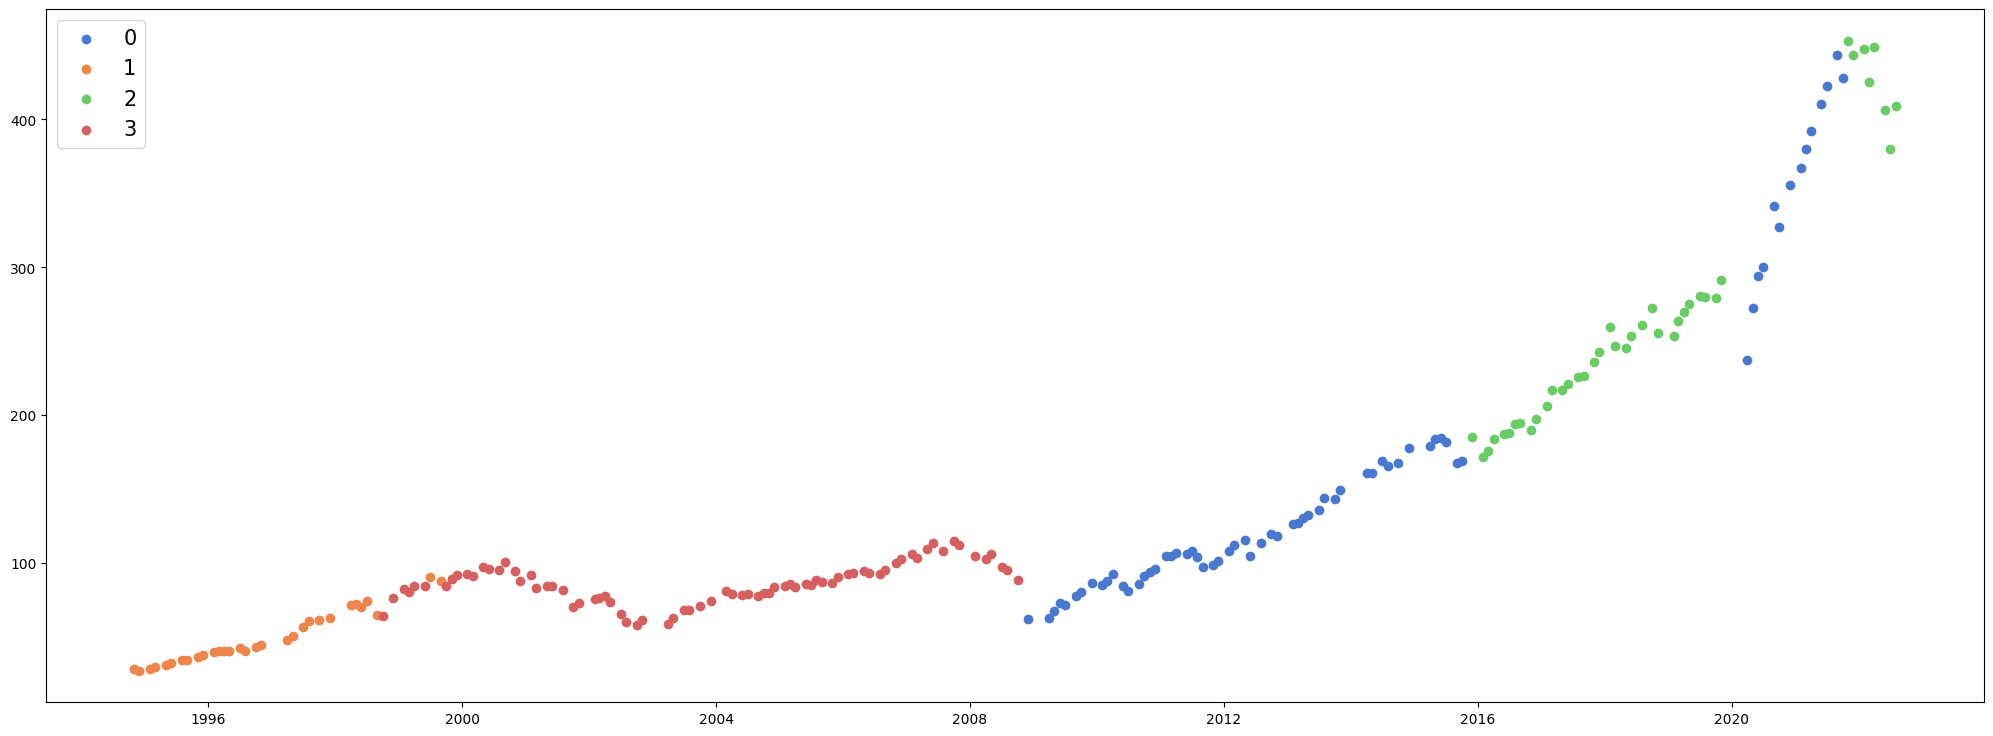
\includegraphics[scale=0.3]{hmm_eco_indic.png}
    \caption{Using HMM to detect Market Regime}\label{hmm_figure}
\end{figure}

\cite{cont_empirical_nodate} proposes that high-volatility events of stocks tend to cluster in time. And according to an \href{https://www.twosigma.com/articles/a-machine-learning-approach-to-regime-modeling/}{article} from Two Sigma, I use GMM to estimate the market regime. The idea is that returns of financial assets do not always follow a normal distribution, GMM fits various Gaussian distributions to capture different parts of the asset’s return distribution, and each of those distributions would have its own properties. I use returns of SPY and its moving average to fit GMM and get best result assuming there're 4 underlying clusters, see figure \ref{gmm_figure}. Although the figure gives a appropriate classification, it's hard to explain green points(state 2) after year 2020.

\begin{figure}[H]
    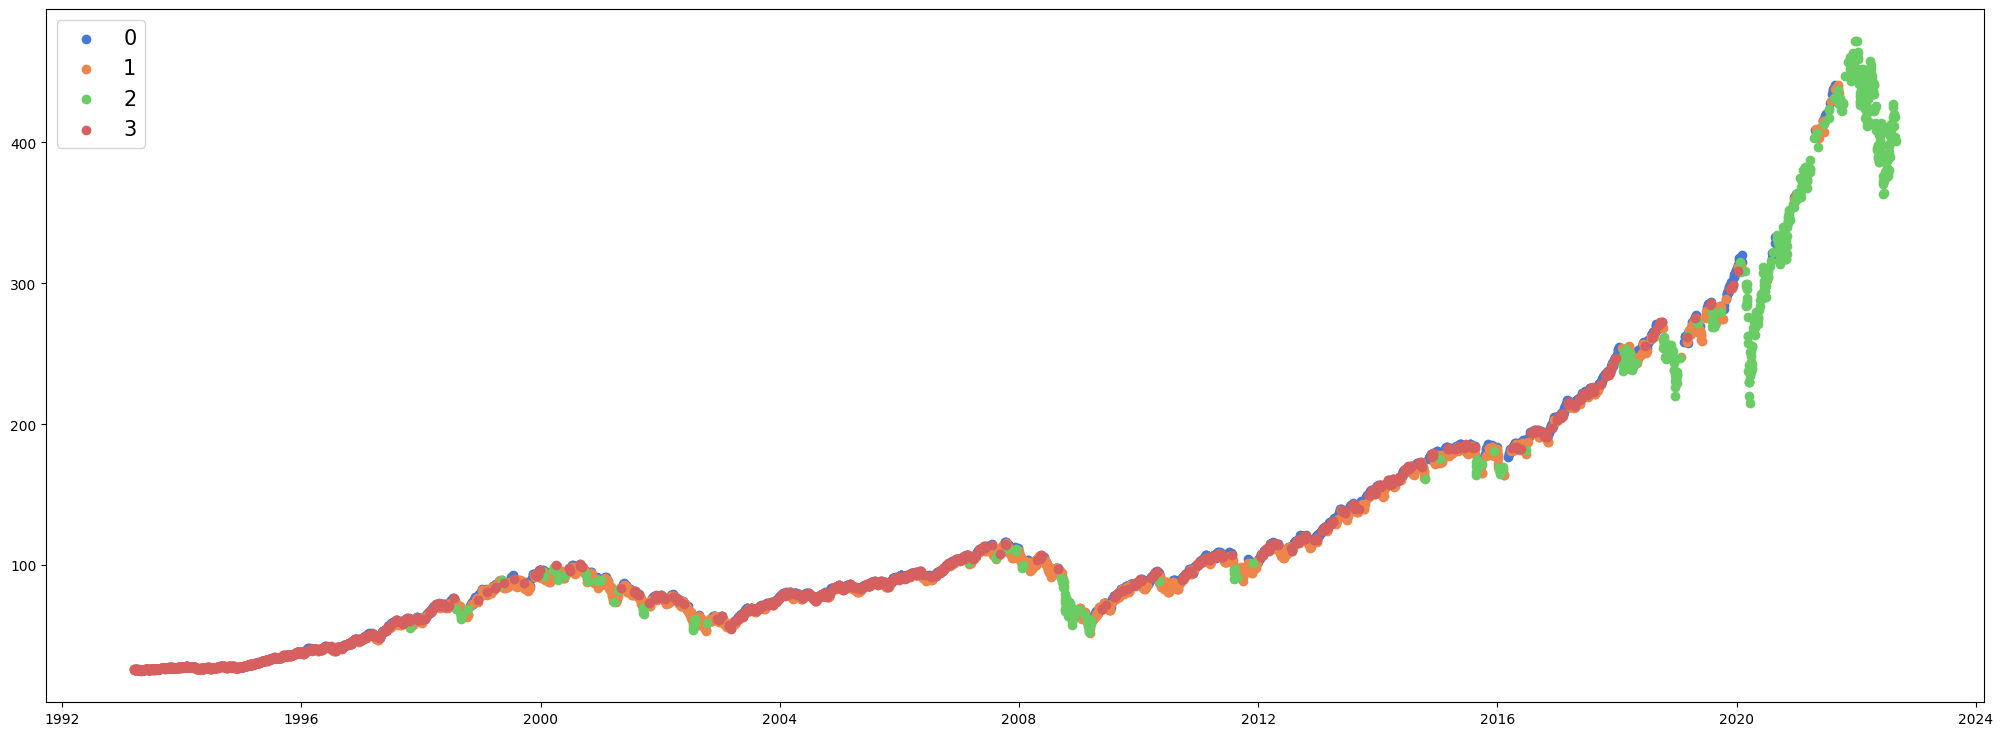
\includegraphics[scale=0.3]{GMM_tech_indic.png}
    \caption{Using GMM to detect Market Regime}\label{gmm_figure}
\end{figure}

Since we know that high-volatility events of stocks tend to cluster in time, another way is to use K-means clustering to classify market regimes. In my test, using SMA, standard deviation, High minus Low, Close minus Open and RSI gives us best result. In each test, I use Elbow plot to determine the number of clusters K, then use K to fit the model. Take my final result as an example, to determine the number of clusters(K), I first create a Elbow plot, see figure \ref{k_clusters}.

\begin{figure}[H]
    \centering
    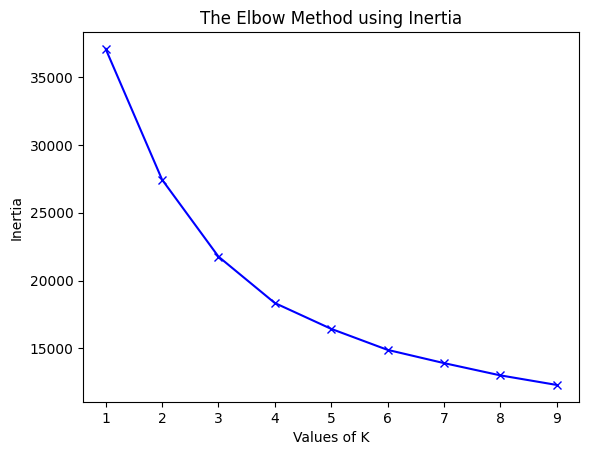
\includegraphics[scale=0.6]{k_clusters.png}
    \caption{Elbow plot of K-means}\label{k_clusters}
\end{figure}

From the figure, we choose to use 4 clusters to fit K-means model, and K-means fits the data perfectly, see figure \ref{kmeans_all}. Figure \ref{kmeans_2008} show a closer result of financial crisis, we find that there's always huge jump around green points (state 2).

\begin{figure}[H]
    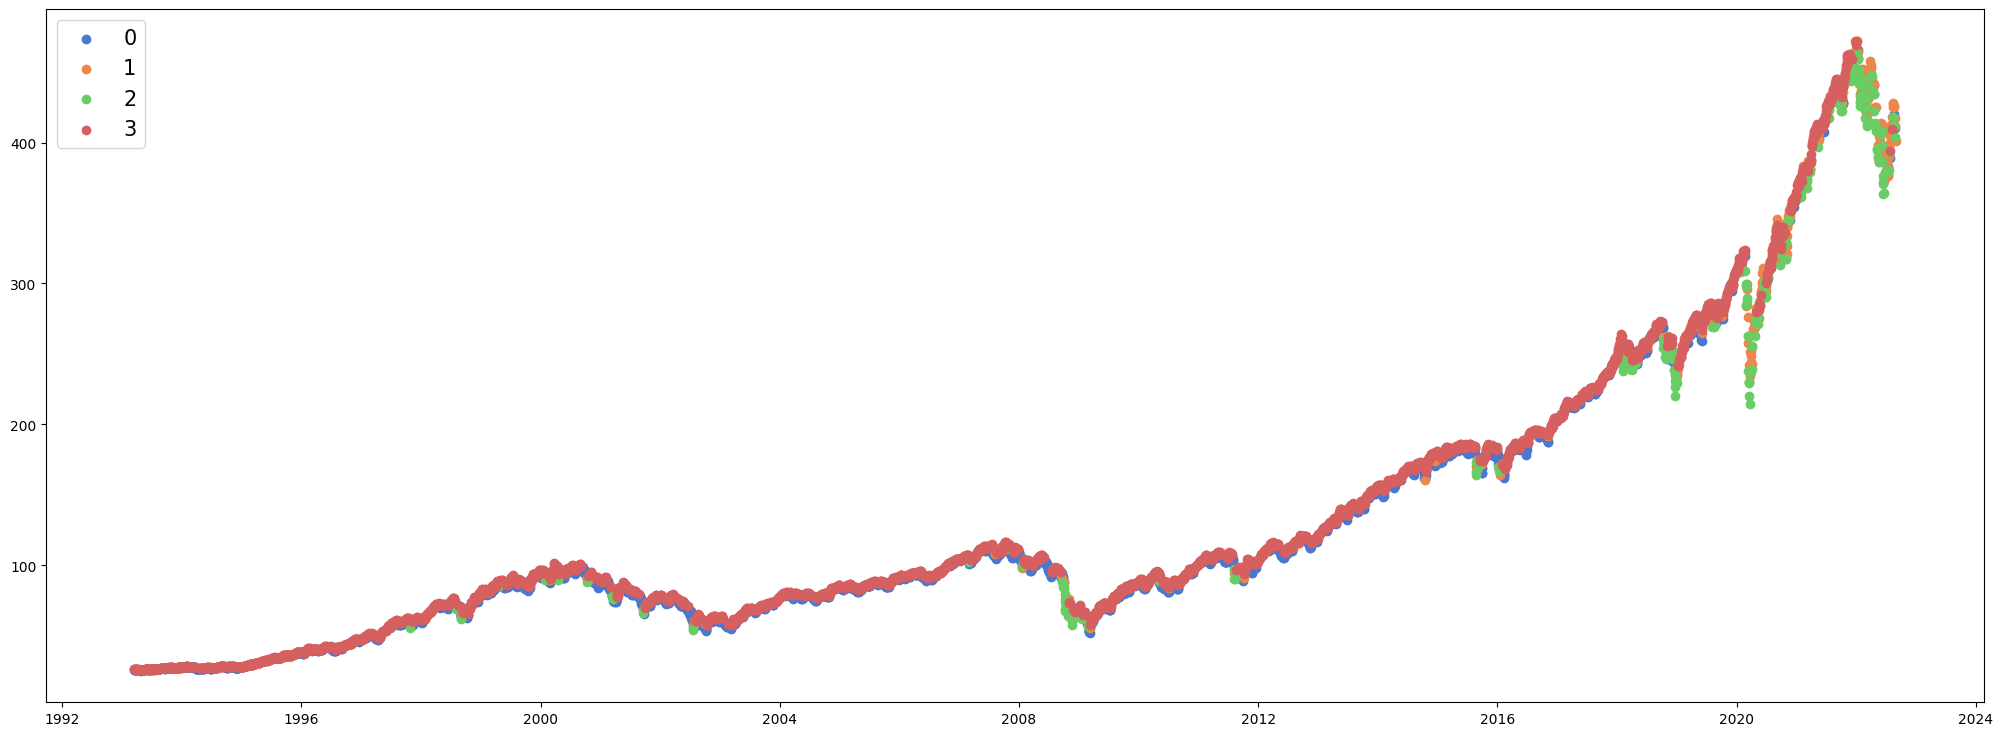
\includegraphics[scale=0.3]{kmeans_all.png}
    \caption{K-means clustering result}\label{kmeans_all}
\end{figure}

\begin{figure}[H]
    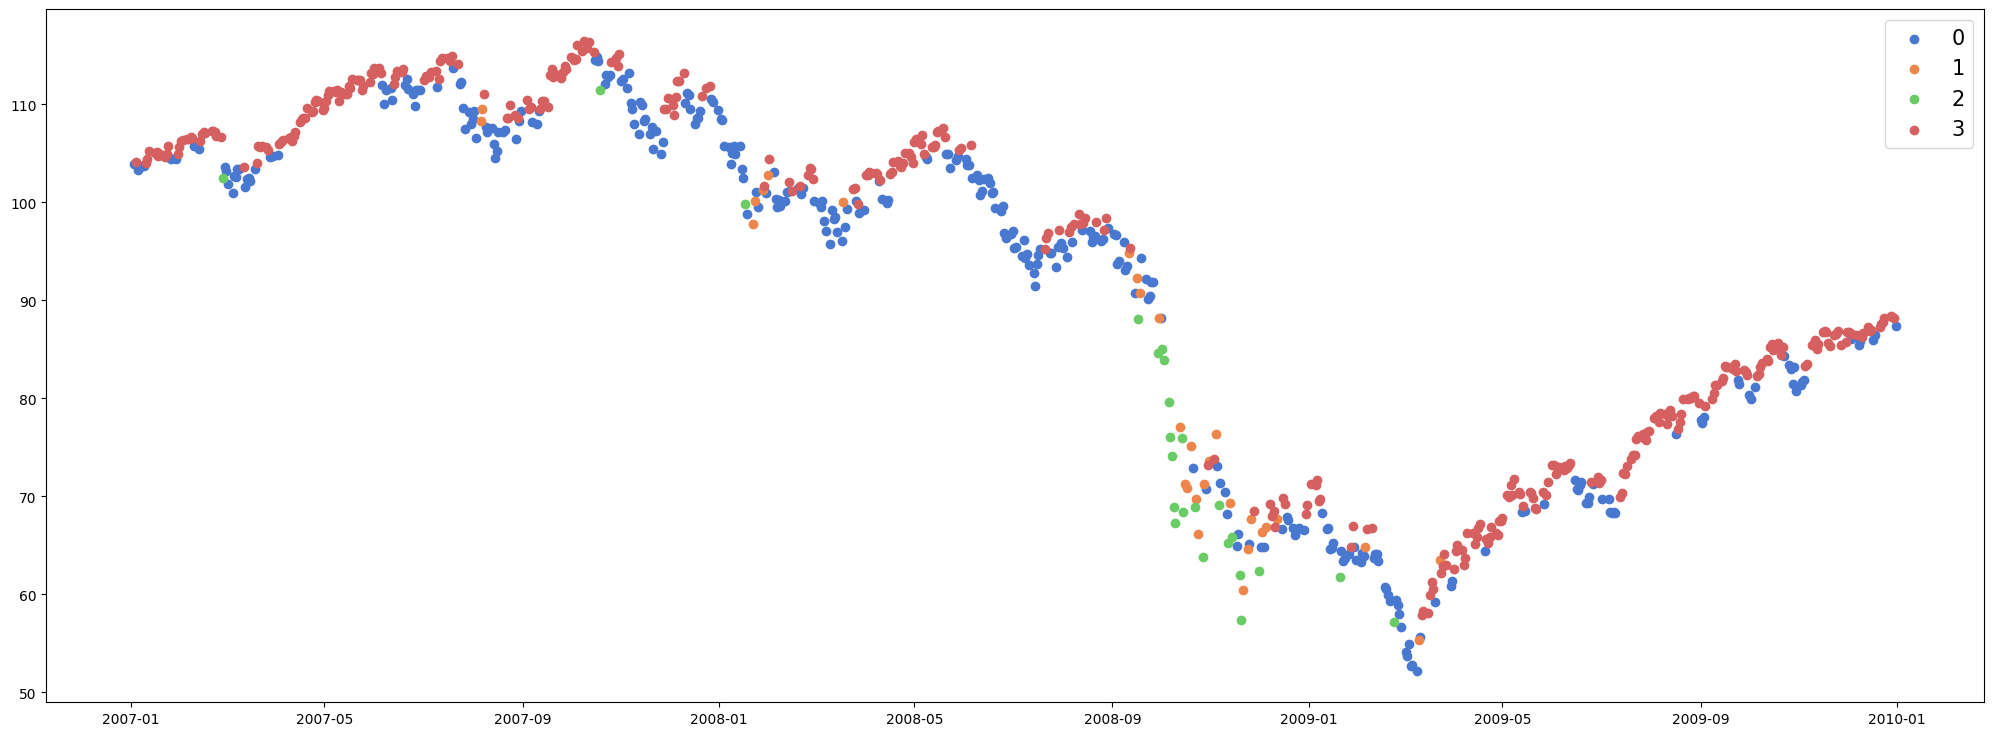
\includegraphics[scale=0.3]{kmeans_2008.png}
    \caption{K-means clustering result during Crisis}\label{kmeans_2008}
\end{figure}

Figure \ref{kmeans_4states} is a figure of 4 states' returns versus standard deviation. It shows that K-means shows four states, where blue points and red points have low standard deviation, orange points and green points have relatively higher standard deviation. And by analyzing their returns, we can conclude that yellow points and green points suggest bull and bear market. Red and blue ones suggest that we are at calm market, but if it's red, the market is more possible to go up. Table \ref{table_4states} verifies our analysis, in which mean and std are calculated by returns of SPY.

\begin{figure}[H]
    \centering
    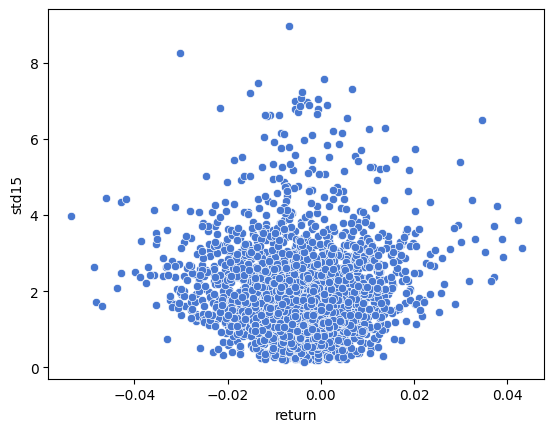
\includegraphics[width=.4\textwidth]{kmeans_0.png}
    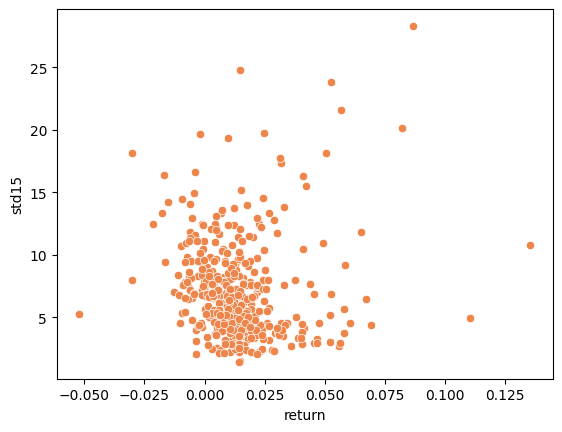
\includegraphics[width=.4\textwidth]{k_means1.png}
    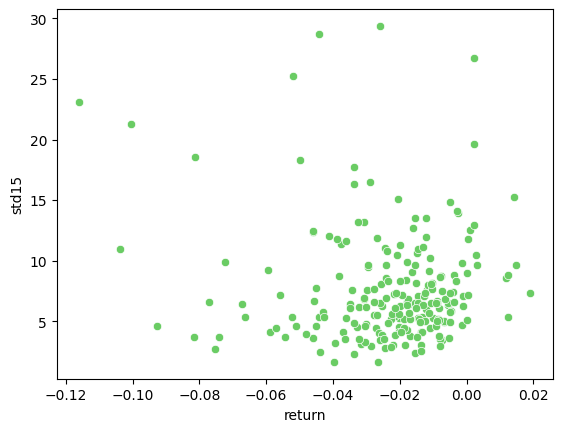
\includegraphics[width=.4\textwidth]{kmeans_2.png}
    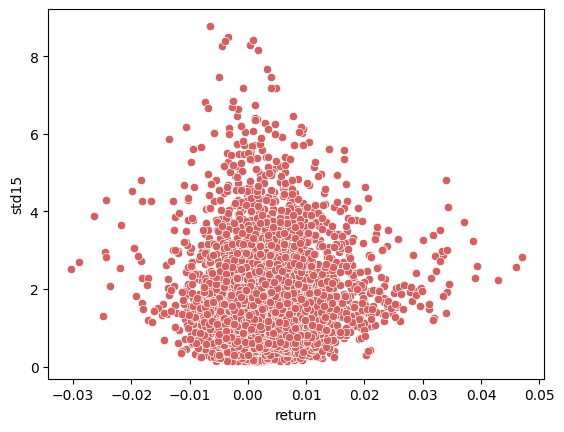
\includegraphics[width=.4\textwidth]{kmeans_3.png}
    \caption{4 regimes}\label{kmeans_4states}
\end{figure}


\subsection{SVM on Stock Selection}

To shrink the number of stocks we invest in, I simply use all the technical indicators to fit the model. The input is all the indicators and output is to determine if the SMA(30 days) two weeks later will be larger than toady's SMA. I test 50 stocks and the prediction accuracy is around 85\%. It's not very high but it's enough for me to get a smaller stock pool.

\section{Backtesting}

In this section, I will do my backtesting based on the research of Chapter \ref{Methodology}. The process of my backtesting is first implementing K-means to detect our current regime, if regime changed, I use SVM to test each stock and select stocks worth investing into my stock pool, then choose an appropriate strategy based on current regime, see the flow chart.

\begin{figure}[H]
    \centering
    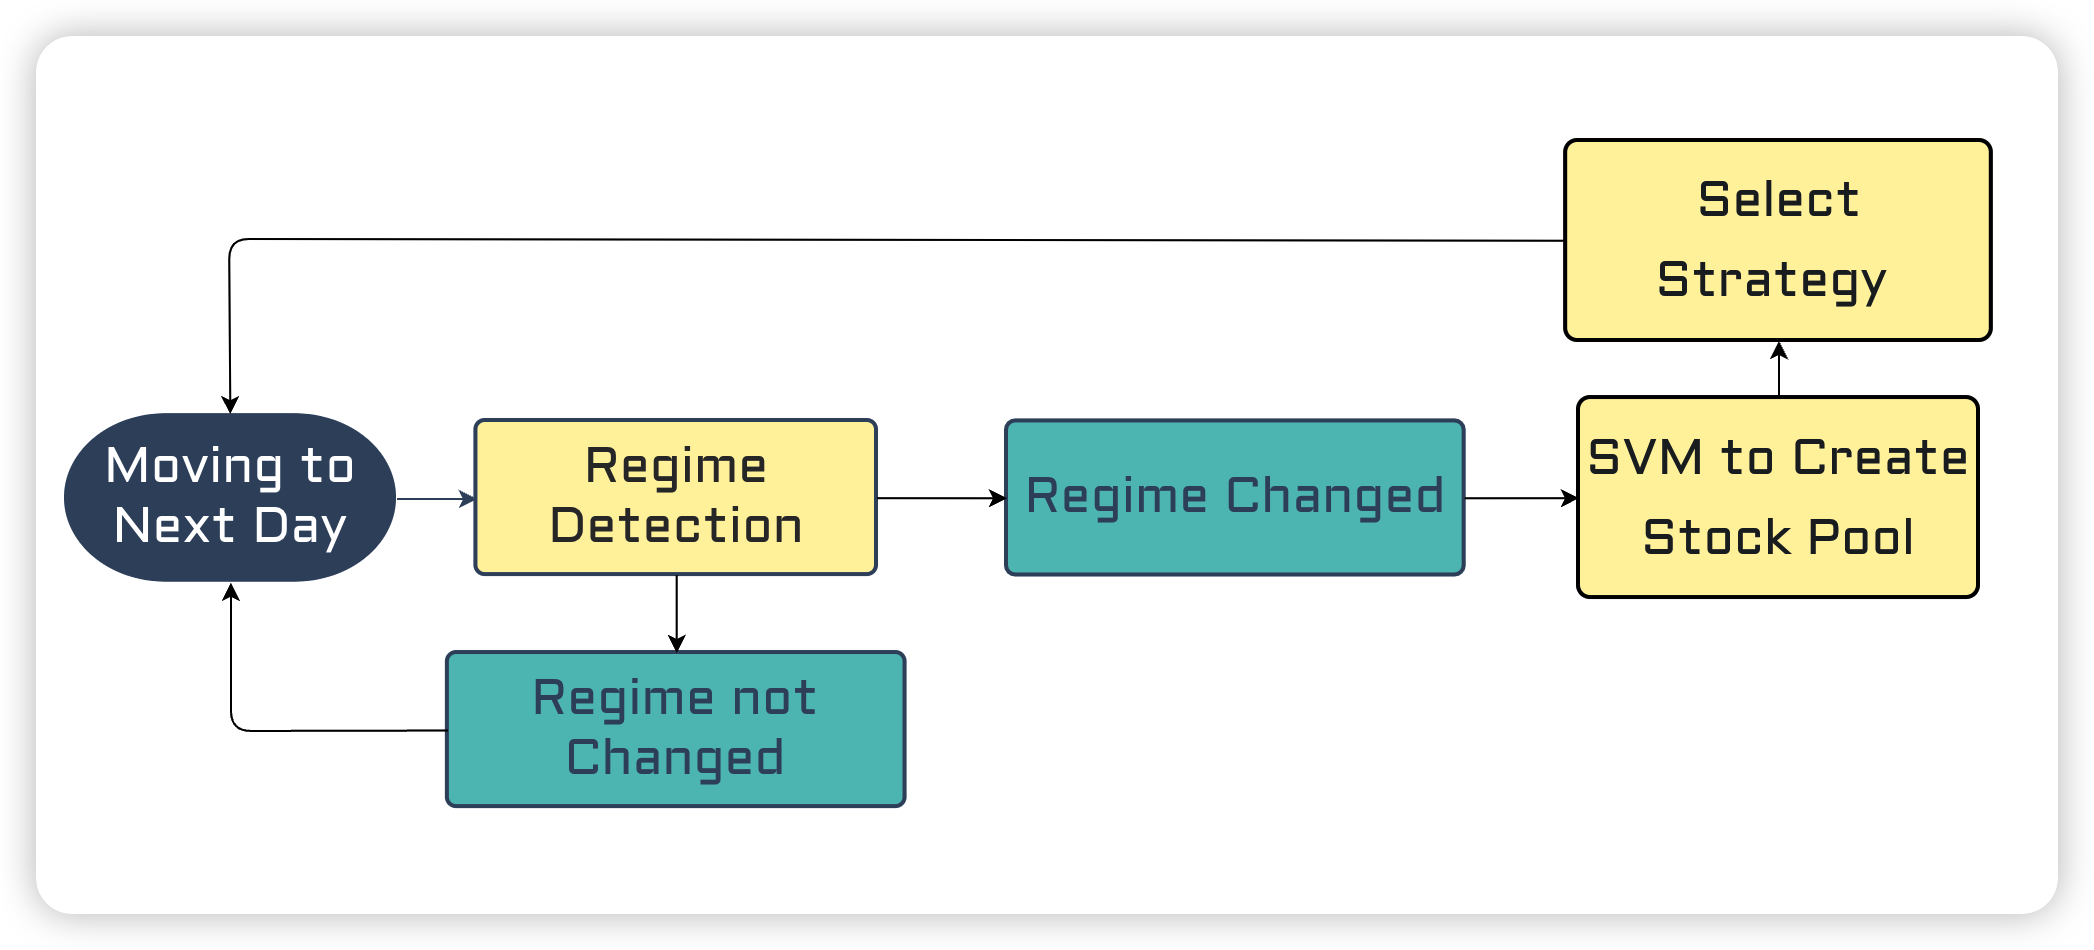
\includegraphics[scale=0.35]{invest.png}
    \caption{Flow Chart}\label{flow_chart}
\end{figure}

In my implementation, I use \href{https://pyportfolioopt.readthedocs.io/en/latest/}{PyPortfolioOpt} built by  \cite{Martin2021} to estimate expected return and covariance matrix with constant correlation shrinkage method. A simple trading strategy is used in my backtesting: 

\begin{enumerate}
    \item If there's a bear market detected within past 2 weeks, I just empty my portfolio.
    \item If there's a clam market detected but with a negative return, I use mean-variance optimization with a relatively high risk-averse parameter.
    \item In other cases, I use maximize the sharpe ratio given sum of all weights equals to 1.
  \end{enumerate}

I set the transaction fee to be 1\%, results are shown in figure \ref{backtest1}. Blue line is my portfolio, green is SPY and orange is equal-weighted portfolio. It doesn't outperform SPY a lot, but we notice that when SPY drops a lot, P\&L of our portfolio doesn't change because we sell all the stocks in advance.

\begin{figure}[H]
    \centering
    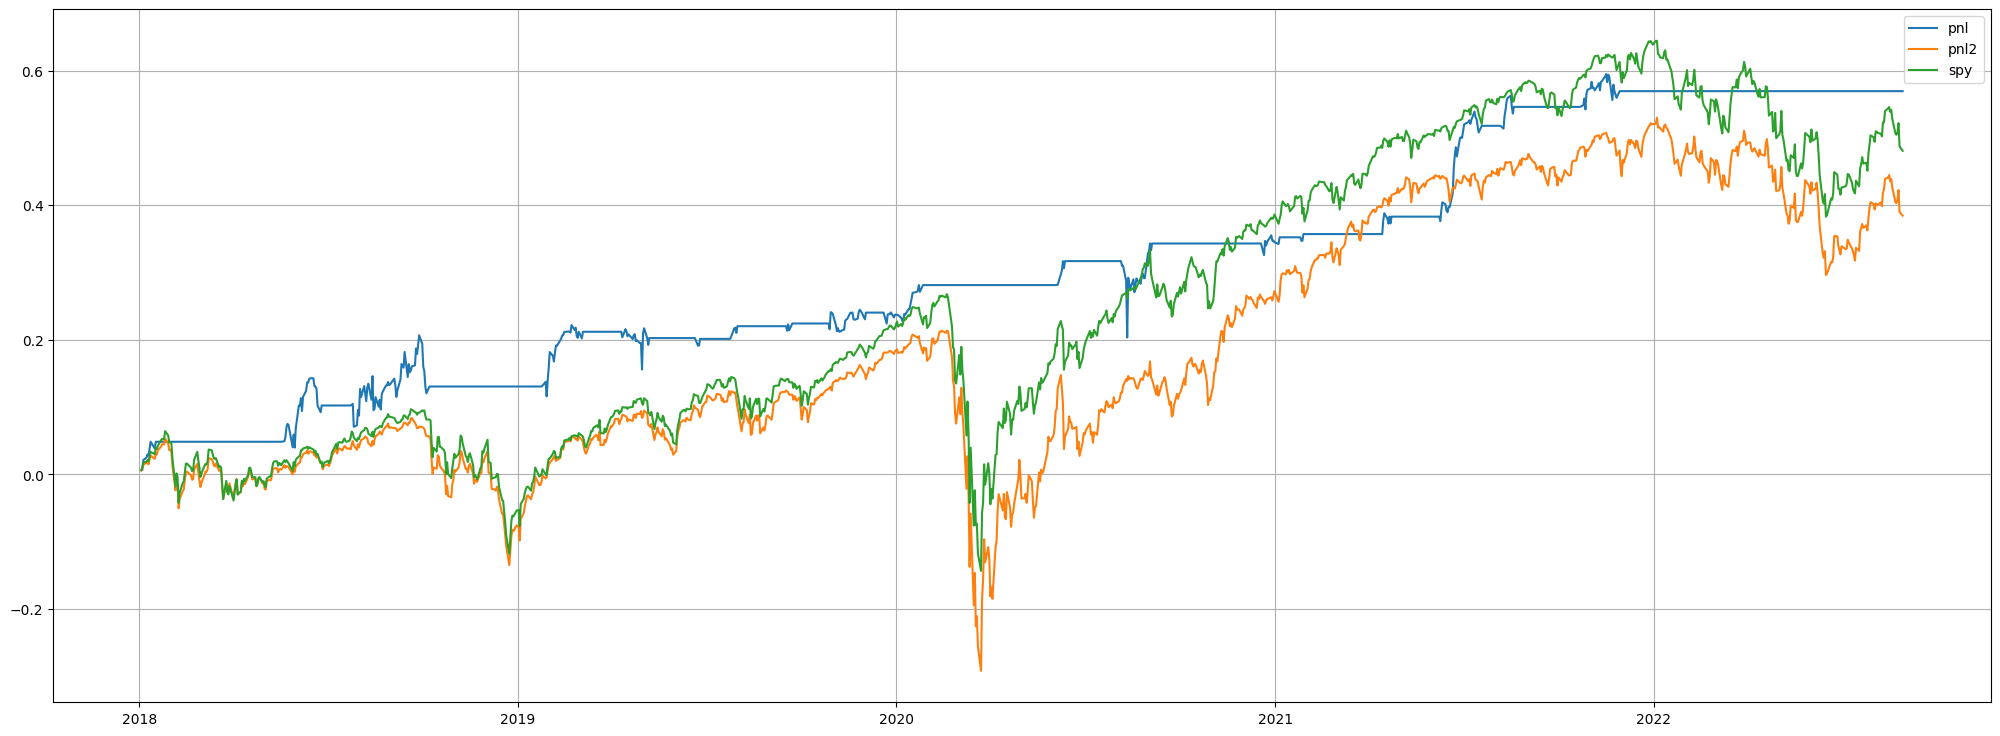
\includegraphics[scale=0.3]{backtest1.png}
    \caption{Backtesing Result}\label{backtest1}
\end{figure}

Indeed, if I relax some constraints of my trading strategy, for example, I only empty my portfolio when there's a bear market detected in 10 days. The performance of my portfolio will be much more better, which benefits from K-means clustering gives me a good result of detecting market regime, see figure \ref{backtest2}. It not only performs better than SPY in bull or calm markets but also avoids huge drops during bear markets.

\begin{figure}[H]
    \centering
    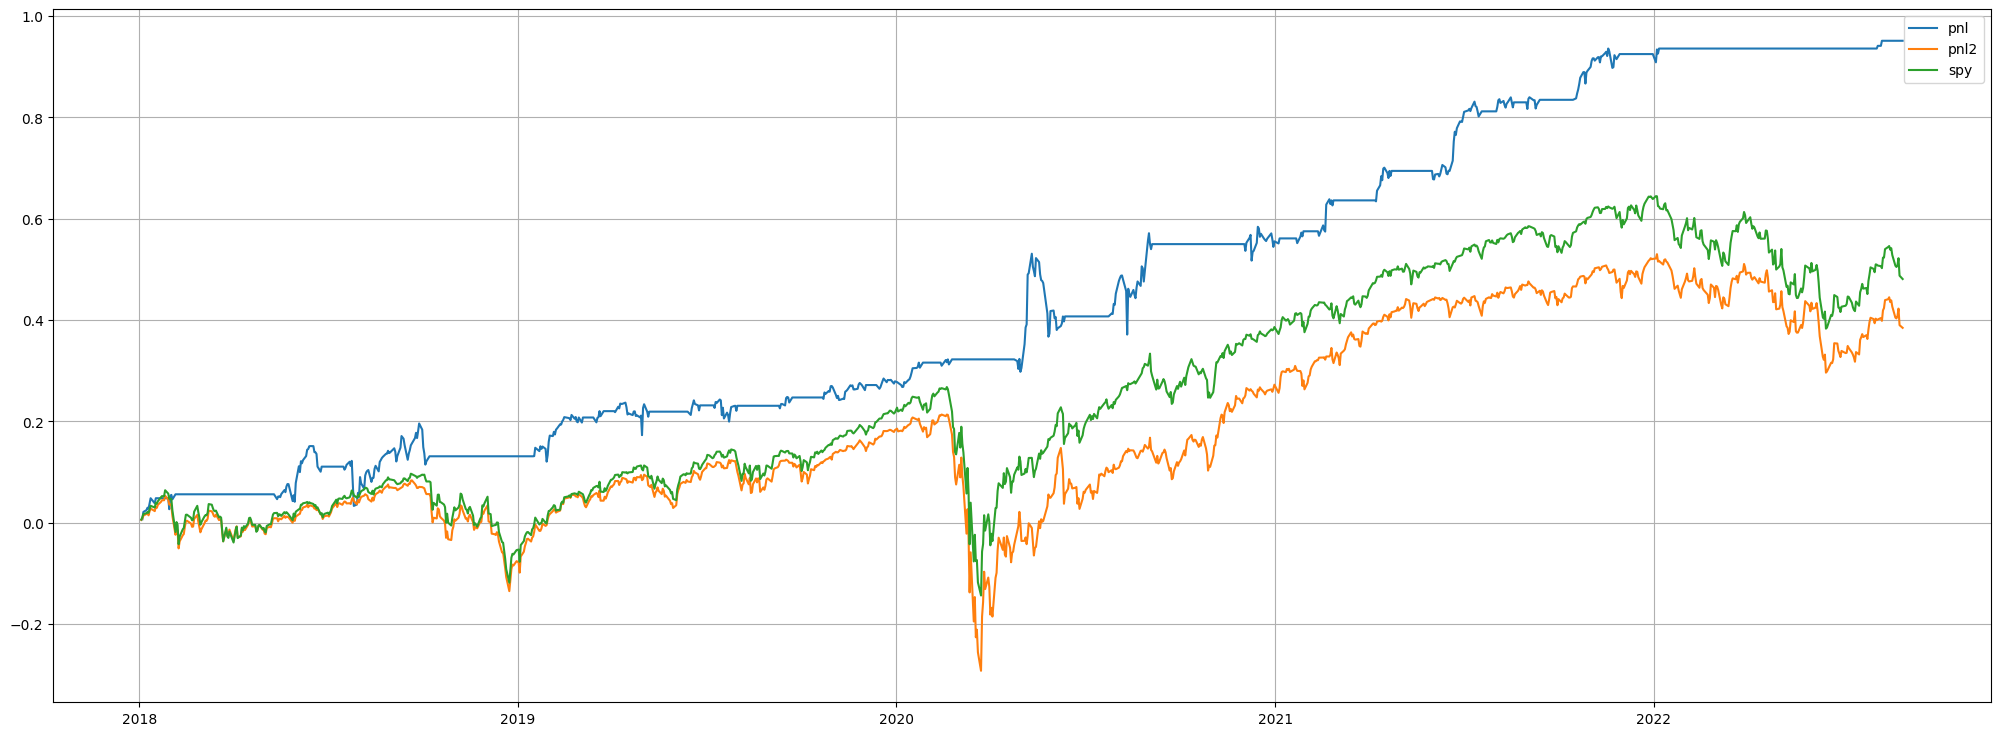
\includegraphics[scale=0.3]{backtest2.png}
    \caption{Backtesing Result 2}\label{backtest2}
\end{figure}

\section{Conclusion}

In my project, I try several ways to detect the regimes of market and find that K-means produces a best result. Based on my market regime model, I built my optimization strategies, results show that they are feasible and efficient.

At the end, there're many future works to do:

\begin{itemize}
    \item In the beginning, I want to build a factor model using auto-encoders as \cite{gu_autoencoder_2021} proposed in his article. However, it requires me a lot of prerequisite knowledge about asset pricing to replicate and modify his method so I give up this idea. And I believe it's interesting to be implemented and the covariance matrix estimation would be more accurate.
    \item The SVM method to determine whether to invest a stock is superficial, and there're many other methods to be investigated. Once I find a more efficient method, the performance of my backtesting result will be better.
    \item Besides, the trading strategy I used in my project can also be improved to get a better result. I think it's also possible to use a deep learning method here, for TD learning or policy gradient.
\end{itemize}

\section{Appendix}

\begin{table}[H]
    \centering
    \begin{tabular}{|l|l|l|l|}
    \hline
    State & Count  & Mean                           & Std                           \\ \hline
    0     & 2428.0 & -0.004335                      & \multicolumn{1}{r|}{1.946686} \\ \hline
    1     & 394    & 0.013764                       & 7.281018                      \\ \hline
    2     & 218    & \multicolumn{1}{r|}{-0.023388} & 7.635582                      \\ \hline
    3     & 4379   & 0.002953                       & \multicolumn{1}{r|}{1.759820} \\ \hline
    \end{tabular}
    \caption{Summary of 4 states}
    \label{table_4states}
\end{table}


\bibliographystyle{chicago}
\bibliography{ref.bib}
\end{document}